\documentclass[11pt,a4paper]{article}
% Scientific Data "Data Descriptor" structure. Port to the journal's LaTeX template
% at submission; section order and headings already follow its author guidelines.
\usepackage[margin=2.4cm]{geometry}
\usepackage{times}
\usepackage{graphicx}
\usepackage{booktabs}
\usepackage{amsmath,amssymb}
\usepackage{url}
\usepackage[hidelinks]{hyperref}
\usepackage{caption}
\usepackage{multirow}
\usepackage{xcolor}
\usepackage[numbers,sort&compress]{natbib}
\sloppy
\captionsetup{font=small,labelfont=bf}
\setlength{\parskip}{0.3em}
% numbers still being produced; every \TBD must be gone before submission
\newcommand{\TBD}[1]{\textcolor{red}{\textbf{[#1]}}}

\title{\textbf{InsightVLM-20K: chart images paired with statistically verified findings}}
\author{A K M Asifuzzman \quad Robiul \quad Fahim Ali \quad Iftehad \quad Md Arfat Yunus\\[0.3em]
\small Group Hocrux, Phitron AI/ML Thesis Track}
\date{}

\begin{document}
\maketitle

\begin{abstract}
\noindent
Charts carry most quantitative findings to readers, yet no public chart corpus pairs an
image with a statement about the plotted data that has been checked to be true.
InsightVLM-20K contains 20{,}000 charts in 26 chart types, each labelled with one of 20
statistical findings such as bimodality, heteroscedasticity or a level shift. A label is
issued only when a named statistical test confirms it on exactly the plotted array and no
other class matches; re-running the tests reproduces 99.95\% of labels. Each sample
carries its data table, statistics, a reasoning chain, a numerically grounded insight and
evidence boxes. 6{,}083 charts come from 654 real public tables in source-disjoint
splits, so generalisation to real data is measured directly. We document a shortcut
audit, a rendering leak we found and removed, and test sets re-drawn by two other
plotting libraries. A fine-tuned CNN ensemble reaches 0.867 on real test charts against
0.468 for the best zero-shot vision--language model, and 0.716 on charts from an unseen
plotting library.
\end{abstract}

% =====================================================================
\section*{Background \& Summary}

Quantitative evidence is usually met as a picture. A reader sees a distribution, a
correlation or a trend long before the numbers behind it, and the properties that most
often invalidate a naive reading, such as two modes behind one mean, variance that
grows with the predictor, or a visible gap between groups that is within sampling
noise, are visible in the figure but rarely stated in its caption.

Chart understanding datasets are mature, but their supervision describes or queries
the chart rather than stating what the data shows. FigureQA\cite{figureqa},
DVQA\cite{dvqa}, PlotQA\cite{plotqa} and ChartQA\cite{chartqa} pair charts with
questions and answers; ChartGen\cite{chartgen} and ChartCoder\cite{chartcoder} pair
them with plotting code; ChartQA-X\cite{chartqax} adds explanations of answers; and
reasoning benchmarks such as CharXiv\cite{charxiv} test description and reasoning
over scientific figures. None attaches a label that a statistical test has confirmed
on the plotted data, so none can be used to train or score a model on whether a
stated finding is \emph{true}.

InsightVLM-20K fills that gap. Its design goals were:
(i) \textbf{verified labels}: a label exists only if a named test confirms it on the
exact plotted array, and only if exactly one class matches;
(ii) \textbf{balance}: exactly 1{,}000 samples per class, split 700/100/200;
(iii) \textbf{measurable generalisation}: real-source charts sit in source-disjoint
splits and are reported separately from synthetic ones;
(iv) \textbf{auditable shortcuts}: every known way to predict the label without
reading the data is measured, and the dataset's own rendering is tested for leaks.

The dataset supports supervised chart classification, vision--language instruction
tuning (instruction/response pairs are included), chart-to-table reconstruction,
and evidence grounding. Because every sample stores its data table and statistics,
it also supports studies of how well models' cited numbers match the data.

% =====================================================================
\section*{Methods}

\subsection*{Finding taxonomy}
Twenty finding classes span four families an analyst routinely reports
(Table~\ref{tab:classes}): six distribution shapes, six relationship types between
two variables, five time-series behaviours and three group or composition findings.
Each class is (i) verifiable by a standard test, (ii) mutually exclusive with the
others by explicit guards, and (iii) visible in at least four chart types.

\begin{table}[t]\centering\small
\caption{The 20 finding classes and the tests that license them.}
\label{tab:classes}
\begin{tabular}{llp{7.6cm}}
\toprule
\textbf{Family} & \textbf{Class} & \textbf{Verification guard} \\
\midrule
\multirow{6}{*}{Distribution}
 & \texttt{dist\_normal}        & Shapiro--Wilk $p>0.05$, $|\text{skew}|<0.35$, dip test\cite{hartigan} $p>0.15$ \\
 & \texttt{dist\_right\_skew}   & skew $>1.0$ and Bowley skew $>0.05$ \\
 & \texttt{dist\_left\_skew}    & skew $<-1.0$ and Bowley skew $<-0.05$ \\
 & \texttt{dist\_bimodal}       & dip $p<0.05$, GMM BIC gain $>10$, KS-uniform $p<0.05$ \\
 & \texttt{dist\_heavy\_tail}   & excess kurtosis $>2.0$, outliers $>2.5\%$, $|$Bowley$|<0.10$ \\
 & \texttt{dist\_uniform}       & KS vs.\ uniform $p>0.10$, excess kurtosis $<-0.9$ \\
\midrule
\multirow{6}{*}{Relationship}
 & \texttt{rel\_strong\_positive}      & Pearson $r>0.70$, $|r-\rho|<0.09$ \\
 & \texttt{rel\_strong\_negative}      & $r<-0.70$, $|r-\rho|<0.09$ \\
 & \texttt{rel\_none}                  & $|r|<0.12$, $|\rho|<0.12$, quadratic $R^2<0.05$ \\
 & \texttt{rel\_nonlinear\_monotonic}  & $|\rho|>0.80$, $|\rho|-|r|>0.10$, linear $R^2<0.72$ \\
 & \texttt{rel\_nonlinear\_nonmono.}   & $|r|<0.25$, quadratic $R^2>0.45$, $|t_{\text{curv}}|>4$ \\
 & \texttt{rel\_heteroscedastic}       & Breusch--Pagan\cite{breuschpagan} $p<0.001$, spread ratio $>2.5$ \\
\midrule
\multirow{5}{*}{Temporal}
 & \texttt{ts\_increasing}    & Mann--Kendall\cite{kendall} $p<0.01$, $\tau>0.35$ \\
 & \texttt{ts\_decreasing}    & Mann--Kendall $p<0.01$, $\tau<-0.35$ \\
 & \texttt{ts\_seasonal}      & periodogram power $>0.30$, ACF $>0.35$, $|\tau|<0.25$ \\
 & \texttt{ts\_changepoint}   & SNR $>2.5$, step model beats line, abruptness $>0.55$ \\
 & \texttt{ts\_anomaly\_spike}& robust $|z|>6$, no trend after removal \\
\midrule
\multirow{3}{*}{Group}
 & \texttt{grp\_significant\_diff} & Kruskal--Wallis\cite{kruskal} $p<0.001$, $\varepsilon^2>0.14$ \\
 & \texttt{grp\_no\_diff}          & Kruskal--Wallis $p>0.30$, $\varepsilon^2<0.02$ \\
 & \texttt{grp\_dominant\_category}& top share $>0.55$, normalised entropy $<0.75$ \\
\bottomrule
\end{tabular}
\end{table}

\subsection*{Verification gate}
Three rules govern labelling. \textbf{Subsample before verifying}: data are reduced to
their final plotted size before any test runs, so the label describes what the image
shows rather than a parent table. \textbf{Exactly one class}: a candidate satisfying
two classes' guards is discarded rather than multi-labelled. \textbf{Reject rather
than mislabel}: every guard is conservative; more candidates can always be mined, a
wrong label cannot be recovered. Robust statistics are used where naive ones fail in
measurable ways: moment skewness alone labelled 12.5\% of symmetric Student-$t(4)$
samples as skewed, so skew classes also require Bowley skewness; the dip test is
calibrated against the uniform, so bimodality also requires a KS test against the
uniform to reject; and a linear ramp produces a high-SNR ``changepoint'', so level
shifts also require a two-level model to beat a line and an abruptness ratio above
0.55. Over 10 seeds $\times$ 20 classes, generators produce their intended class
95.5\% of the time; every miss is a rejection, not a wrong label.

\subsection*{Source data}
\emph{Real track.} We harvested 719 public tables from OpenML\cite{openml}, the World
Bank, Our World in Data, vega-datasets, seaborn-data and UCI, and mined every
plottable view: single columns, column pairs, per-entity time series,
numeric-by-category groupings and categorical compositions. Real data cannot fill
every class: across all 719 tables only 10 clean inverted-U relationships exist.
\emph{Synthetic track.} Data whose property holds by construction were generated with
domain vocabularies (health, economics, environment, engineering, education, retail)
and realistic names, units and magnitudes. Both tracks pass the identical gate.
Provenance is balanced within each class rather than filled real-first, so that no
class is dominated by one provenance. The final corpus has 6{,}083 real samples from
654 source tables (30.4\%) and 13{,}917 synthetic samples.

\subsection*{Splits}
Samples are split 14{,}000/2{,}000/4{,}000 (700/100/200 per class). Real samples are
split by source table: every chart derived from one table is in one split. The real
subsets contain 4{,}338 training, 553 validation and 1{,}192 test charts; real class
frequencies are uneven because public data are (Supplementary Table~S1).

\subsection*{Supplementary real training pool}
The balanced set caps real data at 500 samples per class, which leaves verified real
candidates unused. We release them as an optional training pool: candidates whose
source table the split hash assigns to \emph{train}, with exact duplicates of any
dataset sample removed and at most 400 per class. By construction no validation or
test source table contributes to it (the build asserts this). It adds 2{,}545 real
training charts in nine classes (Supplementary Table~S1), raising real training data
from 4{,}338 to 6{,}883 charts. It is kept separate from the balanced splits.

\subsection*{Rendering}
Charts are drawn with matplotlib\cite{matplotlib} and seaborn\cite{seaborn} on a fixed
$768\times576$ canvas in 26 chart types and 8 visual styles. The style of each sample
is chosen from a CRC32 hash of its identifier, so rendering is reproducible across
processes. Tight bounding-box cropping is disabled, because it resizes the canvas
after the axes transform is read and would shift every evidence box. Dates stored as
epoch timestamps are plotted as calendar dates.

\paragraph{Label-dependent marks were removed (version 2).} The first release drew
annotations on time-series charts that depended on the label: a fitted trend line only
on increasing and decreasing series, a vertical line at the change point only on
level-shift series, and circles only around anomalies. These marks reveal the class
without the data being read, and trained models used them (see Technical Validation).
Version 2 draws no label-dependent marks; the corresponding evidence is kept only as
grounding boxes in the metadata. No other chart family drew label-dependent marks
(regression lines on scatter plots are drawn independently of the label).
Figure~\ref{fig:marks} shows both renders of the same data.

\begin{figure}[t]\centering
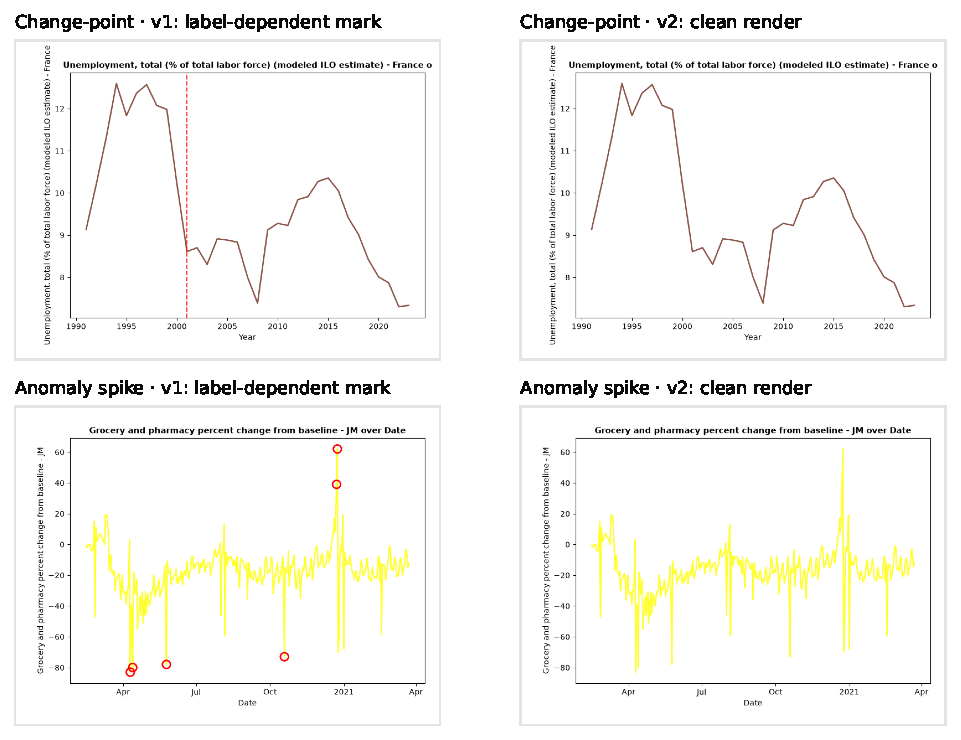
\includegraphics[width=\linewidth]{../figures/fig_marks_examples.pdf}
\caption{The same real data rendered with the version-1 label-dependent mark (left)
and in the released version-2 form (right). Top: a level shift in French unemployment;
bottom: anomalies in a mobility series.}
\label{fig:marks}
\end{figure}

\subsection*{Cross-renderer test sets}
To test whether models learn matplotlib's appearance rather than the statistics, all
1{,}192 real test tables were re-drawn with two further libraries. \emph{Plotly}\cite{plotly}
differs in fonts, gridlines, colours, marker shapes, binning rules and layout; five
templates are assigned by hash, excluding the one that imitates seaborn.
\emph{Vega-Lite} (rendered with vl-convert) uses nine themes, excluding those that
match a matplotlib training style. Chart types map to each library's nearest native
form; where none exists (for example boxen or hexbin plots) the substitute is a form
the taxonomy lists as valid for every class that chart type can carry. No
label-dependent marks are drawn.

\subsection*{Training-only renderer augmentation}
For training we additionally release two alternative renders of every training and
supplementary chart: a Plotly render, and a matplotlib render with randomised fonts,
font sizes, line and marker sizes, colours, background tints, gridlines, spines and
title placement (data and chart type unchanged). No validation or test chart is
rendered this way, and no Vega-Lite render is used for training, so Vega-Lite remains
a renderer that no model has seen.

\subsection*{Additional annotations}
Each sample stores the plotted data table, a statistics dictionary (moments, quantiles,
correlation coefficients, test statistics, $p$-values and effect sizes), the name of
the test that licensed its label, a reasoning chain (observation $\rightarrow$
statistic $\rightarrow$ test $\rightarrow$ conclusion), an insight paragraph in which
every claim cites a computed number, and pixel boxes for the plot area and the
supporting evidence (for example the modal bin, the outlier band, the change point or
the dominant wedge).

% =====================================================================
\section*{Data Records}

The dataset is deposited at \TBD{Zenodo/Figshare DOI} under CC BY 4.0 and mirrored on
Kaggle (\url{https://www.kaggle.com/datasets/asifxzaman/insightvlm-20k-v2}).
Table~\ref{tab:files} lists the files.

\begin{table}[t]\centering\small
\caption{Files in the release.}
\label{tab:files}
\begin{tabular}{p{4.6cm}p{10.2cm}}
\toprule
\textbf{Path} & \textbf{Contents} \\
\midrule
\texttt{images/<class>/<id>.png} & 20{,}000 chart images, $768\times576$ RGBA PNG \\
\texttt{records.jsonl} & one JSON record per sample: identifiers, label, family, chart type, split, provenance, source and licence, data table, statistics, test, reasoning chain, insight, render metadata and evidence boxes \\
\texttt{tables/metadata.parquet} & the same fields flattened for analysis \\
\texttt{splits/\{train,val,test\}.jsonl} & records per split \\
\texttt{splits/test\_real\_only.jsonl} & the 1{,}192 real-source test samples \\
\texttt{instruct/\{split\}.jsonl} & image/prompt/response triples for instruction tuning \\
\texttt{test\_renders/\{plotly,vega\}/} & Plotly and Vega-Lite re-renders of the 1{,}192 real test charts \\
\texttt{train\_extra/} & supplementary real training pool: 2{,}545 images and \texttt{records\_extra.jsonl} \\
\texttt{train\_aug/\{plotly,mplrand\}/} & alternative renders of every training and supplementary chart \\
\texttt{class\_index.json} & label $\leftrightarrow$ id map, class descriptions, valid chart types, tests \\
\texttt{DATASHEET.md}, \texttt{BIAS\_AUDIT.md} & datasheet\cite{datasheets} and audit report \\
\bottomrule
\end{tabular}
\end{table}

Sample identifiers have the form \texttt{<class>\_\_<index>}. Provenance is
\texttt{real} or \texttt{synthetic}; real samples record their source repository,
source table identifier, URL and licence. Difficulty (\texttt{easy/medium/hard}) is
the within-class tertile of the evidence margin, i.e.\ how far the deciding statistic
lies beyond its guard.

% =====================================================================
\section*{Technical Validation}

\subsection*{Label correctness and integrity}
Re-running the verification battery on each test sample's stored data table
reproduces 3{,}998 of 4{,}000 labels (0.9995); the two exceptions lie within 1\% of the
heteroscedasticity guard and fail to \emph{no class} rather than to a wrong class under
a different \texttt{statsmodels} build. The integrity audit finds 0 of 654 source
tables in more than one split, 0 duplicate data fingerprints and one visual duplicate
among 20{,}000 images.

\subsection*{Shortcut audit}
A shortcut is any feature that predicts the label without the statistical evidence.
Eleven were measured on version 2 against thresholds fixed in advance, and all pass
(Table~\ref{tab:bias}). Real and synthetic charts are not separable from low-level
pixel statistics (AUC 0.551), so the synthetic majority does not give provenance
away. Chart type is associated with the label by construction (a pie chart can only
carry a composition finding); we disclose this and use it as the evaluation floor
rather than removing it.

\begin{table}[t]\centering\small
\caption{Shortcut audit on version 2. All eleven tests pass.}
\label{tab:bias}
\begin{tabular}{lrr}
\toprule
\textbf{Test} & \textbf{Value} & \textbf{Threshold} \\
\midrule
Class balance (imbalance ratio)                    & 1.000  & $=1.000$ \\
Split balance (max s.d.\ of class proportions)     & 0.0000 & $<0.01$ \\
Chart type $\rightarrow$ label (prior accuracy)    & 0.2883 & reported as floor \\
Render style $\rightarrow$ label (Cram\'er's $V$)  & 0.0000 & $<0.05$ \\
Provenance detectability from pixels (AUC)         & 0.551  & $<0.75$ \\
Axis text $\rightarrow$ label (macro-F1)           & 0.3688 & $<0.55$ \\
Pixel statistics $\rightarrow$ label (macro-F1)    & 0.4038 & $<0.55$ \\
Source concentration (top share in a class)        & 17.2\% & $<35\%$ \\
Length confound within family (ratio)              & 2.04   & $<4.0$ \\
Subject-domain concentration                       & 22.8\% & $<45\%$ \\
Category-vocabulary concentration                  & 13.0\% & $<35\%$ \\
\bottomrule
\end{tabular}
\end{table}

\subsection*{A rendering leak, measured and removed}
The shortcut audit examines metadata and pixel statistics, not what a trained model
attends to, and it did not detect the version-1 time-series marks. We found them by
inspecting the renderer and measured their effect directly: the same 1{,}000 test time
series were rendered twice with identical styles, once with the marks and once
without, and scored with two ResNets trained on version 1 (Figure~\ref{fig:ablation}).
With marks, accuracy on real time series was 0.957 (ResNet-101) and 0.944
(ResNet-50); without them it fell to 0.311 and 0.407, with the level-shift class
dropping from 1.000 to 0.355. Seasonal series, the one temporal class that carried no
mark, were unaffected (0.97 in both renders). Zero-shot vision--language models, which
never saw version-1 training data, changed by only 1--2.5 points on all real charts
and 4--10 points on real time series. This is shortcut learning\cite{geirhos} in its plainest form, and we report
it because version-1 results in earlier drafts of this work overstated real-data
accuracy. All results below use version 2.

\begin{figure}[t]\centering
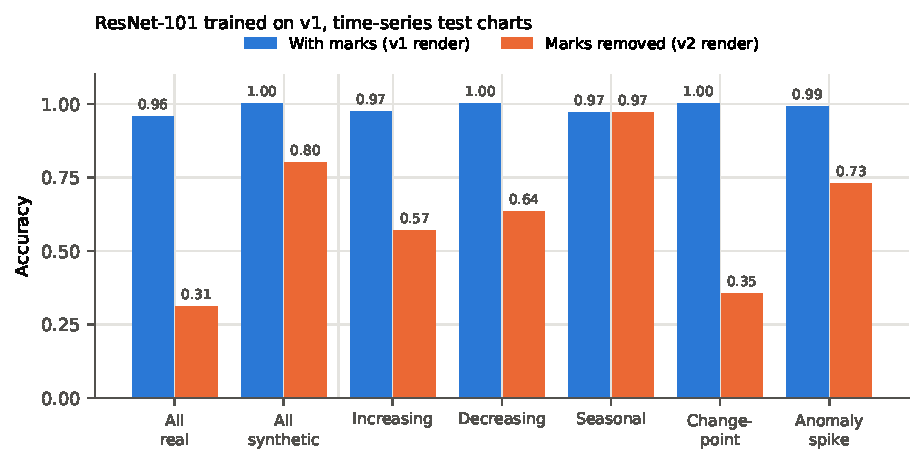
\includegraphics[width=\linewidth]{../figures/fig_marks_ablation.pdf}
\caption{Accuracy of a ResNet-101 trained on version 1 on test time series rendered
with and without the label-dependent marks. Only the marks differ between the two
renders.}
\label{fig:ablation}
\end{figure}

\subsection*{Evidence grounding}
A Grad-CAM pointing game on the 1{,}023 real test charts that carry evidence boxes checks
whether the deployed models attend to the evidence that licenses each label. The
attention peak falls inside an evidence box on 52.4\% of charts against 43.9\% for a
random point in the plot area (gain $+8.5$ points, 95\% CI $[+6.8, +10.2]$): clearly for
time series ($+15.4$) and group comparisons ($+11.0$), less for relationships ($+7.3$),
and not for distributions ($-0.2$). The evidence boxes are therefore usable as a
grounding reference for three of the four families.

\subsection*{Evaluation protocol}
With 20 balanced classes chance is 5\%, but a rule that uses no pixels, predicting
the most common class for each chart type, reaches 0.288; we use it as the floor. A
data oracle that runs the verification battery on the stored table reaches 0.9995 and
is the ceiling. The headline metric is accuracy on the 1{,}192 real test charts, with
95\% bootstrap confidence intervals\cite{efron}; paired differences between systems
are tested with exact McNemar tests\cite{mcnemar} on the same charts. Mixed-test
accuracy is reported for completeness but is dominated by synthetic charts.

\subsection*{Baselines}
\paragraph{Fine-tuned CNNs.} ResNet-101 and ResNet-50\cite{resnet} and
DenseNet-121\cite{densenet}, ImageNet-initialised, were trained at $384\times384$ for
up to 12 epochs (AdamW, one-cycle schedule, label smoothing 0.1). Horizontal and
vertical flips are never used: mirroring converts a positive correlation into a
negative one and an increasing series into a decreasing one. Batches are sampled so
that about half are real charts, and the checkpoint is chosen on real validation
accuracy. Members are trained on the balanced training split, on the split plus the
supplementary pool, and on the latter with renderer augmentation (each epoch shows each
training chart as one of its three renders, uniformly). The deployed ensemble is the equal-weight average of the models trained
with the full recipe (supplementary pool and renderer augmentation); only a label-shift
correction\cite{saerens} towards real-data class frequencies is tuned, on validation.
Membership was set after all models were trained, so we also report the alternatives:
averaging every trained model gives 0.862 on real test charts, and greedy ensemble
selection\cite{caruana} on validation gives 0.865. With 553 real validation charts,
greedy selection chases one- to two-point differences that do not reliably transfer.

\paragraph{Zero-shot vision--language models.} Qwen2.5-VL-3B and 7B\cite{qwen25vl} and
Qwen3-VL-8B\cite{qwen3vl} received each chart with all 20 class names and one-line
definitions and were asked for one class name, with greedy decoding. All three
produced a parseable class for more than 99.9\% of charts. They were evaluated on the
matplotlib renders only.

\paragraph{Human annotators.} A human baseline on 200 real test charts (10 per class; 2
for the inverted-U class) has been deployed as a web form that shows each chart with the
20 findings in plain language, in a different random order per annotator, with anonymous
chart identifiers. It had no valid submission at the time of writing and will be reported
with the published dataset.

\begin{table}[t]\centering\small
\caption{Accuracy on the 1{,}192 real test charts drawn by three renderers, and on
synthetic test charts. Brackets: 95\% bootstrap CI. $^\dagger$Fixed 400-chart synthetic
sample.}
\label{tab:results}
\resizebox{\linewidth}{!}{%
\begin{tabular}{lcccc}
\toprule
 & \multicolumn{3}{c}{\textbf{Real test charts}} & \\
\cmidrule(lr){2-4}
\textbf{System} & \textbf{matplotlib} & \textbf{Plotly} & \textbf{Vega-Lite} & \textbf{Synthetic} \\
\midrule
Chart-type prior (no pixels)            & \multicolumn{4}{c}{0.288 (all test charts)} \\
Qwen2.5-VL-3B, zero-shot                & 0.306 [0.281, 0.332] & -- & -- & 0.303$^\dagger$ \\
Qwen2.5-VL-7B, zero-shot                & 0.411 [0.383, 0.440] & -- & -- & 0.498$^\dagger$ \\
Qwen3-VL-8B, zero-shot                  & 0.468 [0.439, 0.496] & -- & -- & 0.648$^\dagger$ \\
\midrule
ResNet-101, balanced split              & 0.841 & 0.747 & 0.607 & 0.997 \\
\quad + supplementary real pool        & 0.840 & 0.735 & 0.602 & 0.999 \\
\quad + renderer augmentation          & 0.859 & 0.854 & 0.650 & 0.998 \\
DenseNet-121, + supplementary pool      & 0.861 & 0.771 & 0.638 & 0.997 \\
\quad + renderer augmentation          & 0.855 & 0.852 & 0.712 & 0.998 \\
\textbf{Ensemble of the two full-recipe models} & \textbf{0.867} [0.846, 0.886] & \textbf{0.857} [0.836, 0.877] & \textbf{0.716} [0.690, 0.741] & \textbf{0.999} \\
\midrule
Statistical oracle (ceiling)            & \multicolumn{4}{c}{0.9995 (all test charts)} \\
\bottomrule
\end{tabular}}
\end{table}

Table~\ref{tab:results} and Figure~\ref{fig:results} summarise the baselines. The deployed
ensemble, the equal-weight average of the two full-recipe models, reaches 0.867 on real
test charts and 0.999 on synthetic ones. Every zero-shot vision--language model is far
below it (best 0.468; exact McNemar $p<10^{-100}$ for each pairwise comparison), and the
weakest, Qwen2.5-VL-3B, is barely above the 0.288 no-pixel floor: naming a statistical
finding from a chart is not something current general-purpose VLMs do reliably without
task-specific training.

Rendering matters as much as data. Trained on matplotlib alone, models lose 8.5--10.6 points
on Plotly re-renders of the same data and 22--25 points on Vega-Lite. Adding the
supplementary real pool changes real accuracy by less than a point for ResNet-101, but
training-only renderer augmentation closes most of the Plotly gap (a renderer it has
seen) and, more tellingly, lifts accuracy on Vega-Lite, which no model has seen, from
0.60--0.64 to 0.65--0.71 without costing matplotlib accuracy. A residual 15-point
unseen-renderer gap remains and is the main open problem the dataset exposes.

Errors concentrate in the distribution family (0.763 on real charts, versus 0.886--0.930
for the other families) and in classes with few real examples: heavy tails (0.385,
$n=26$), seasonality (0.462, $n=13$) and left skew (0.474, $n=19$). The commonest
confusions are between classes that differ in degree rather than kind: bimodal read as
right-skewed (19 of 100), heavy-tailed read as right-skewed (13 of 26), and significant
group differences read as none (12 of 100). Macro-F1 on real charts is 0.776.

\begin{figure}[t]\centering
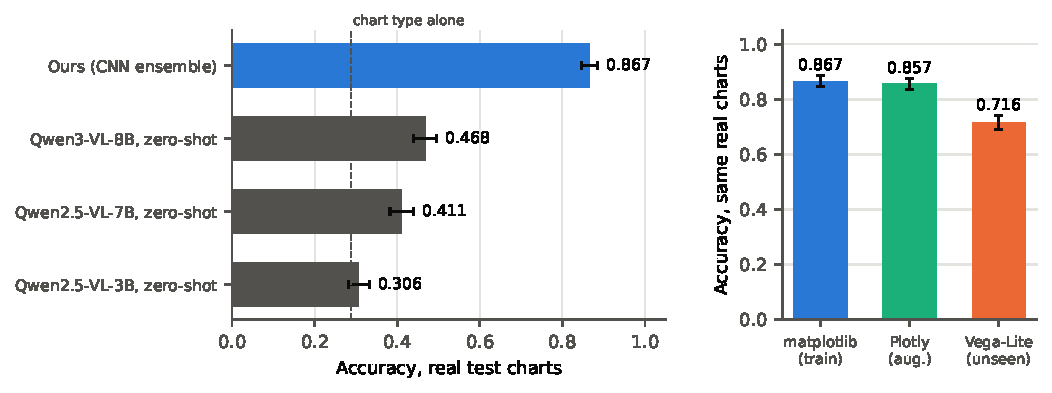
\includegraphics[width=\linewidth]{../figures/fig_results.pdf}
\caption{Left: accuracy on the 1{,}192 real test charts (matplotlib renders), 95\%
bootstrap CIs; dashed line, the chart-type prior. Right: the deployed ensemble on the
same real charts drawn by the training renderer, by Plotly (used only as training
augmentation) and by Vega-Lite (never seen).}
\label{fig:results}
\end{figure}

% =====================================================================
\section*{Usage Notes}

\begin{itemize}\itemsep0.2em
\item \textbf{Report real-only accuracy.} The corpus is 70\% synthetic, and
synthetic charts are easier; mixed accuracy hides the generalisation gap. Use
\texttt{splits/test\_real\_only.jsonl}.
\item \textbf{Report an unseen renderer.} Score the Vega-Lite re-renders of the real
test charts, and do not train on Vega-Lite. If the Plotly training renders are used for
augmentation, the Plotly test renders measure a seen renderer and should be labelled so.
\item \textbf{Report against the floor, not 5\%.} Chart type alone gives 0.288.
\item \textbf{Do not flip images.} Horizontal or vertical flips change the label for
roughly 30\% of samples.
\item \textbf{Tune on validation only.} Real validation has 553 charts; selecting
models or ensembles on the test split inflates results (an earlier draft of this work
did so).
\item \textbf{Single label.} Charts showing two findings at once were excluded, so
models trained here will not report compound findings.
\item \textbf{Thresholds are conventions.} $|r|>0.7$ for ``strong'' or
$\varepsilon^2>0.14$ for ``large'' follow common practice; every guard is recorded in
\texttt{class\_index.json} and the verification code, so labels can be re-derived
under other choices.
\item \textbf{Class priors are artificial.} Balance is a training convenience;
real-world finding frequencies are skewed. The real subsets reflect public-data
frequencies.
\end{itemize}

% =====================================================================
\section*{Code Availability}
The complete pipeline (harvesting, mining, synthesis, the verification battery,
rendering, validation, export, the shortcut audit, the Plotly renderer, training
notebooks, ensembling, statistics and figures) is available at \TBD{repository URL}.
The corpus rebuilds end to end in under an hour on a laptop CPU.

% =====================================================================
\section*{Author Contributions}
\TBD{Contributions per author.}

\section*{Competing Interests}
The authors declare no competing interests.

\clearpage
\section*{Supplementary Information}
\begin{table}[h]\centering\small
\caption*{\textbf{Supplementary Table S1.} Real-source samples per class and split, and in the supplementary training pool (train-split sources only). Synthetic samples fill each class to 700/100/200 in the balanced splits.}
\begin{tabular}{lrrrr}
\toprule
\textbf{Class} & \textbf{Train} & \textbf{Val} & \textbf{Test} & \textbf{Supplementary} \\
\midrule
\texttt{dist\_normal} & 126 & 16 & 21 & -- \\
\texttt{dist\_right\_skew} & 350 & 50 & 100 & 208 \\
\texttt{dist\_left\_skew} & 48 & 8 & 19 & -- \\
\texttt{dist\_bimodal} & 350 & 50 & 100 & 400 \\
\texttt{dist\_heavy\_tail} & 116 & 21 & 26 & -- \\
\texttt{dist\_uniform} & 74 & 19 & 21 & -- \\
\texttt{rel\_strong\_positive} & 240 & 42 & 84 & -- \\
\texttt{rel\_strong\_negative} & 45 & 9 & 14 & -- \\
\texttt{rel\_none} & 350 & 50 & 100 & 400 \\
\texttt{rel\_nonlinear\_monotonic} & 118 & 29 & 42 & -- \\
\texttt{rel\_nonlinear\_nonmonotonic} & 6 & 1 & 2 & -- \\
\texttt{rel\_heteroscedastic} & 350 & 50 & 100 & 143 \\
\texttt{ts\_increasing} & 350 & 50 & 100 & 400 \\
\texttt{ts\_decreasing} & 350 & 8 & 100 & 140 \\
\texttt{ts\_seasonal} & 47 & 4 & 13 & -- \\
\texttt{ts\_changepoint} & 145 & 4 & 26 & -- \\
\texttt{ts\_anomaly\_spike} & 350 & 5 & 66 & 237 \\
\texttt{grp\_significant\_diff} & 350 & 50 & 100 & 245 \\
\texttt{grp\_no\_diff} & 350 & 50 & 100 & 372 \\
\texttt{grp\_dominant\_category} & 223 & 37 & 58 & -- \\
\midrule
\textbf{Total} & 4,338 & 553 & 1,192 & 2,545 \\
\bottomrule
\end{tabular}
\end{table}


\bibliographystyle{unsrtnat}
\bibliography{references}

\end{document}
